\documentclass{article}
\usepackage{tikz}
\usepackage{float}
\usepackage{enumerate}
\usepackage{amsmath}
\usepackage{bm}
\usepackage{indentfirst}
\usepackage{siunitx}
\usepackage[utf8]{inputenc}
\usepackage{graphicx}
\graphicspath{ {Images/} }
\usepackage{float}
\allowdisplaybreaks

\title{8.01 Problem Set 9}
\author{Robert Durfee - Lecture 7 - Table 9}
\date{November 7, 2017}

\begin{document}

\maketitle

\section{Moment of Inertia: Disc and Washer}

\subsection*{Part A}

\begin{enumerate}[i]
    \item Axis passing through the center of mass.
    \begin{figure}[H]
        \centering
        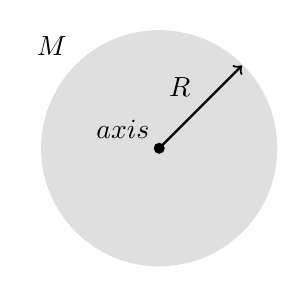
\begin{tikzpicture}
            \fill [gray!25!white] (0,0) circle (1.5);
            \draw [thick, ->] (0,0) -- (1.05,1.05) node[pos=0.5, anchor=south east]{$R$};
            \draw (-1.05,1.05) node[anchor=south east]{$M$};
            \fill (0,0) circle (2pt) node[anchor=south east]{$axis$};
        \end{tikzpicture}
    \end{figure}
    General definition of moment of inertia:
    $$I=\int\limits_{M} r^{2}dm$$
    Define an areal density equation:
    $$\sigma=\frac{M}{\pi R^{2}}$$
    Define a small area, $dA$, of the disk:
    \begin{figure}[H]
        \centering
        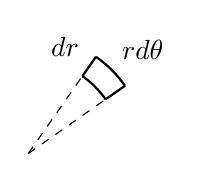
\begin{tikzpicture}
            \draw [dashed] (0,0) -- (1.22873,0.860365);
            \draw [dashed] (0,0) -- (0.860365,1.22873);
            \draw [thick] (1.22873,0.860365) arc (35:55:1.5) node[pos=0.5,
                anchor=south west]{$rd\theta$};
            \draw [thick] (0.98298,0.688292) arc (35:55:1.2);
            \draw [thick] (1.22873,0.860365) -- (0.98298,0.688292);
            \draw [thick] (0.860365,1.22873) -- (0.688292,0.98298) node[pos=0.5,
                anchor=south east]{$dr$};
        \end{tikzpicture}
    \end{figure}
    Its mass, $dm$, can then be written as:
    $$dm=\sigma rdrd\theta$$
    Substitute into the general definition of moment of inertia:
    \begin{align*}
        I&=\int\limits_{0}^{2\pi}\int\limits_{0}^{R}\sigma r^{3} drd\theta\\
        I&=\sigma\left(\int\limits_{0}^{R}r^{3}dr\right)\left(\int\limits_{0}^{2\pi}d\theta\right)\\
        I&=\sigma\left(\left.\frac{r^{4}}{4}\right\vert^{R}_{0}\right)\left(\left.\theta\right\vert^{2\pi}_{0}\right)\\
        I&=\frac{2\pi\sigma R^{4}}{4}
    \end{align*}
    Substitute $\sigma$:
    \begin{align*}
        I&=\frac{2\pi M R^{4}}{4\pi R^{2}}\\
        \bm{I}&\bm{=\frac{1}{2}M R^{2}}
    \end{align*}
    
    \item Axis passing through a point on the rim of the disc a distance $R$
        from the center.
    \begin{figure}[H]
        \centering
        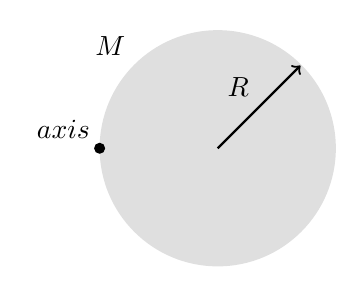
\begin{tikzpicture}
            \fill [gray!25!white] (0,0) circle (1.5);
            \draw [thick, ->] (0,0) -- (1.05,1.05) node[pos=0.5, anchor=south
                east]{$R$};
            \draw (-1.05,1.05) node[anchor=south east]{$M$};
            \fill (-1.5,0) circle (2pt) node[anchor=south east]{$axis$};
        \end{tikzpicture}
    \end{figure}
    The same definitions for $dm$ and $\sigma$ hold, however, the limits of
    integration change.
    \begin{align*}
        I&=\int\limits_{-\pi/2}^{\pi/2}\int\limits_{0}^{2R\cos(\theta)}\sigma
        r^{3} drd\theta\\
        I&=\sigma\int\limits_{-\pi/2}^{\pi/2}\left[\int\limits_{0}^{2R\cos(\theta)}r^{3}
    dr\right]d\theta\\
        I&=\sigma\int\limits_{-\pi/2}^{\pi/2}\left[\left.\frac{r^{4}}{4}\right\vert^{2R\cos(\theta)}_{0}\right]d\theta\\
        I&=4\sigma R^4\int\limits_{-\pi/2}^{\pi/2}\cos^{4}(\theta)d\theta\\
        I&=\sigma R^4\int\limits_{-\pi/2}^{\pi/2}(1+\cos(2\theta))^{2}d\theta\\
        I&=\sigma R^4\int\limits_{-\pi/2}^{\pi/2}(1+2\cos(2\theta)+\cos^{2}(2\theta))d\theta\\
        I&=\frac{\sigma R^4}{2}\int\limits_{-\pi/2}^{\pi/2}(3+4\cos(2\theta)+\cos(4\theta))d\theta\\
        I&=\frac{\sigma
R^4}{8}\left.\left[12\theta+8\sin(2\theta)+\sin(4\theta)\right]\right\vert^{\pi/2}_{-\pi/2}\\
        I&=\frac{\sigma
        R^4}{8}\left[\left(6\pi+8\sin(\pi)+\sin(2\pi)\right)-\left(-6\pi-8\sin(\pi)-\sin(2\pi)\right)\right]\\
        I&=\frac{\sigma R^4}{4}\left(6\pi+8\sin(\pi)+\sin(2\pi)\right)\\
        I&=\frac{3\pi\sigma R^4}{2}
    \end{align*}
    Substitute $\sigma$:
    \begin{align*}
        I&=\frac{3\pi M R^4}{2\pi R^{2}}\\
        \bm{I}&\bm{=\frac{3}{2} M R^2}
    \end{align*}
    
\end{enumerate}

\subsection*{Part B}
    \begin{figure}[H]
        \centering
        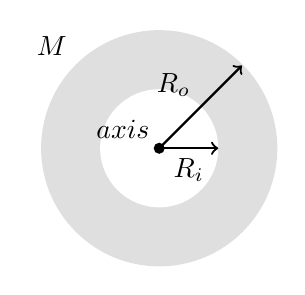
\begin{tikzpicture}
            \fill [gray!25!white] (0,0) circle (1.5);
            \fill [white] (0,0) circle (0.75);
            \draw [thick, ->] (0,0) -- (1.05,1.05) node[pos=0.5, anchor=south east]{$R_o$};
            \draw [thick, ->] (0,0) -- (0.75,0) node[pos=0.5, anchor=north]{$R_i$};
            \draw (-1.05,1.05) node[anchor=south east]{$M$};
            \fill (0,0) circle (2pt) node[anchor=south east]{$axis$};
        \end{tikzpicture}
    \end{figure}
    The same definition of $dm$ holds, however, the definition of $\sigma$ and
    the limits of integration change. Define an areal density equation:
    $$\sigma=\frac{M}{\pi (R^{2}_{o}-R^{2}_{i})}$$
    
    \begin{align*}
        I&=\int\limits_{0}^{2\pi}\int\limits_{R_i}^{R_o}\sigma r^{3}drd\theta\\
        I&=\sigma\left(\int\limits_{R_i}^{R_o}r^{3}dr\right)\left(\int\limits_{0}^{2\pi}d\theta\right)\\
        I&=\sigma\left(\left.\frac{r^{4}}{4}\right\vert^{R_o}_{R_i}\right)\left(\left.\theta\right\vert^{2\pi}_{0}\right)\\
        I&=\frac{2\pi\sigma (R^{4}_{o}-R^{4}_{i})}{4}
    \end{align*}
    Substitute $\sigma$:
    \begin{align*}
        I&=\frac{2\pi M (R^{4}_{o}-R^{4}_{i})}{4\pi (R^{2}_{o}-R^{2}_{i})}\\
        I&=\frac{1}{2}M (R^{2}_{o}+R^{2}_{i})
    \end{align*}
    Given that the volume density $\rho=7.8\cdot10^{3}\ \si{kg\ m^{-3}}$, calculate mass $M$:
    \begin{align*}
        \rho&=\frac{M}{\pi d(R^{2}_{o}-R^{2}_{i})}\\
        M&=\pi \rho d(R^{2}_{o}-R^{2}_{i})
    \end{align*}
    Substitute into moment of inertia equation:
    \begin{align*}
        I&=\frac{1}{2}M (R^{2}_{o}+R^{2}_{i})\\
        I&=\frac{1}{2}\pi \rho d(R^{4}_{o}-R^{4}_{i})
    \end{align*}
    Substitute $R_{i}=13.5\ \si{mm}$, $R_{o}=31.0\ \si{mm}$, $d=4.0\ \si{mm}$, and $\rho=7.8\cdot10^{3}\ \si{kg\ m^{-3}}$:
    \begin{align*}
        I&=\frac{1}{2}\pi (7.8\cdot10^{3}\ \si{kg\ m^{-3}}) (0.004\ \si{m})((0.0310\ \si{m})^{4}-(0.0135\ \si{m})^{4})\\
        \bm{I}&\bm{=4.363\cdot 10^{-5}}\ \si{kg\ m^{-3}}
    \end{align*}
    
\section{Compound Pulley}
    \begin{figure}[H]
        \centering
        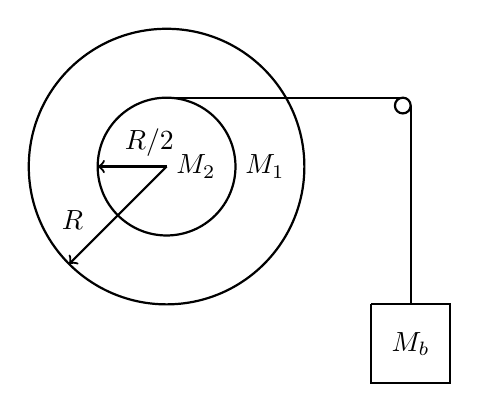
\begin{tikzpicture}
            \draw [thick] (0,0) circle (0.875);
            \draw [thick] (0,0) circle (1.75);
            \draw [thick, ->] (0,0) -- (-1.237,-1.237) node[pos=0.75,
                anchor=south east]{$R$};
            \draw [thick, ->] (0,0) -- (-0.875,0) node[pos=0.25,
                anchor=south]{$R/2$};
            \draw [thick] (0,0.875) -- (3,0.875);
            \draw [thick] (3,0.775) circle (0.1);
            \draw [thick] (3.1,0.775) -- (3.1,-1.75);
            \draw [thick] (2.6,-1.75) -- (3.6,-1.75) -- (3.6,-2.75) --
                (2.6,-2.75) -- (2.6,-1.75);
            \draw (3.1, -2.25) node[]{$M_b$};
            \draw (0,0) node[anchor=west]{$M_2$};
            \draw (0.875,0) node[anchor=west]{$M_1$};
        \end{tikzpicture}
    \end{figure}
Derive the moment of inertia of the compound pulley by summing the moments of
inertia of the two independent pulleys using calculations completed in the last
problem for uniform discs.
\begin{alignat*}{2}
    I_{1}&=\frac{1}{2}MR^{2}&&=\frac{1}{2}M_{1}R^{2}\\
    I_{2}&=\frac{1}{2}MR^{2}&&=\frac{1}{8}M_{2}R^{2}\\
    I_{T}&=\frac{1}{2}M_{1}R^{2}+\frac{1}{8}M_{2}R^{2}&&=\frac{1}{8}(4M_{1}+M_{2})R^{2}
\end{alignat*}
Draw free body diagrams for the forces acting on the pulley and the block:
    \begin{figure}[H]
        \centering
        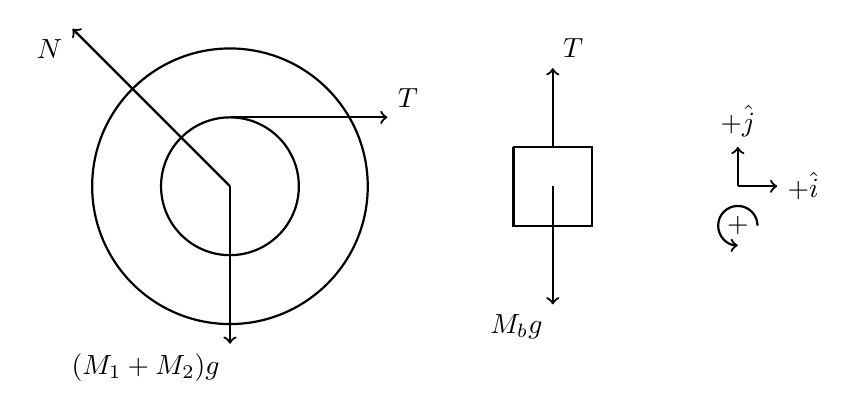
\begin{tikzpicture}
            \draw [thick] (0,0) circle (0.875);
            \draw [thick] (0,0) circle (1.75);
            \draw [thick, ->] (0,0.875) -- (2,0.875) node[pos=1, anchor=south
                west]{$T$};
            \draw [thick, ->] (0,0) -- (0,-2) node[pos=1,anchor=north
                east]{$(M_{1}+M_{2})g$};
            \draw [thick, ->] (0,0) -- (-2,2) node[pos=1,anchor=north
                east]{$N$};
            \draw [thick] (3.6,0.5) -- (4.6,0.5) -- (4.6,-0.5) -- (3.6,-0.5) --
                (3.6,0.5);
            \draw [thick, ->] (4.1,0) -- (4.1, -1.5) node[pos=1, anchor=north
                east]{$M_bg$};
            \draw [thick, ->] (4.1,0.5) -- (4.1, 1.5) node[pos=1, anchor=south
                west]{$T$};
            \draw [thick, ->] (6.45,0) -- (6.45,0.5)
                node[anchor=south]{$+\hat{j}$};
            \draw [thick, ->] (6.45,0) -- (6.95,0)
                node[anchor=west]{$+\hat{i}$};
            \draw [thick, ->] (6.7,-0.5) arc (0:270:0.25);
            \draw (6.45,-0.50) node[]{+};
        \end{tikzpicture}
    \end{figure}

Write out Newton's 2nd Law for the pulley and the block:
\begin{gather}
    -T(R/2)\hat{k}+g(M_1+M_2)(0)\hat{k}+N(0)\hat{k}=\frac{2I_Ta}{R}\hat{k}\\
    \vec{T}+(M_1+M_2)\vec{g}+\vec{N}=0\\
    -M_bg\hat{j}+T\hat{j}=M_ba\hat{j}
\end{gather}

Using equations 1 and 3, we can solve for $a$:
\begin{align*}
    M_ba+M_bg&=-\frac{4I_Ta}{R^{2}}\\
    \left(M_b+\frac{4I_T}{R^{2}}\right)a&=-M_bg\\
    a&=-\frac{M_bgR^{2}}{M_bR^{2}+4I_T}
\end{align*}

Now that we know the acceleration, we can solve for distance travelled in a
certain time:
\begin{align*}
    d&=\frac{1}{2}at^{2}\\
    d&=\frac{M_bR^{2}gt^{2}}{2M_bR^{2}+8I_T}
\end{align*}
Substituting for $I_{T}$ so the answer is in terms of $M_{1}$ and $M_{2}$:
\begin{align*}
    d&=\frac{M_bR^{2}gt^{2}}{2M_bR^{2}+8I_T}\\
    d&=\frac{M_bR^{2}gt^{2}}{2M_bR^{2}+(4M_{1}+M_{2})R^{2}}\\
    d&=\frac{M_bgt^{2}}{2M_b+(4M_{1}+M_{2})}
\end{align*}
Rearrange to solve for $t$:
\begin{align*}
    d&=\frac{M_bgt^{2}}{2M_b+(4M_{1}+M_{2})}\\
    t^{2}&=d\left(\frac{2M_b+4M_{1}+M_{2}}{gM_b}\right)\\
    \bm{t}&\bm{=\sqrt{d\left(\frac{2M_b+4M_{1}+M_{2}}{gM_b}\right)}}
\end{align*}

\section{Massive Pulleys and Moving Blocks}

\begin{figure}[H]
    \centering
    \includegraphics[scale=0.55]{"Figure 1"}
\end{figure}

Draw free-body diagrams for the forces acting on the pulleys and the blocks:

\begin{figure}[H]
    \centering
    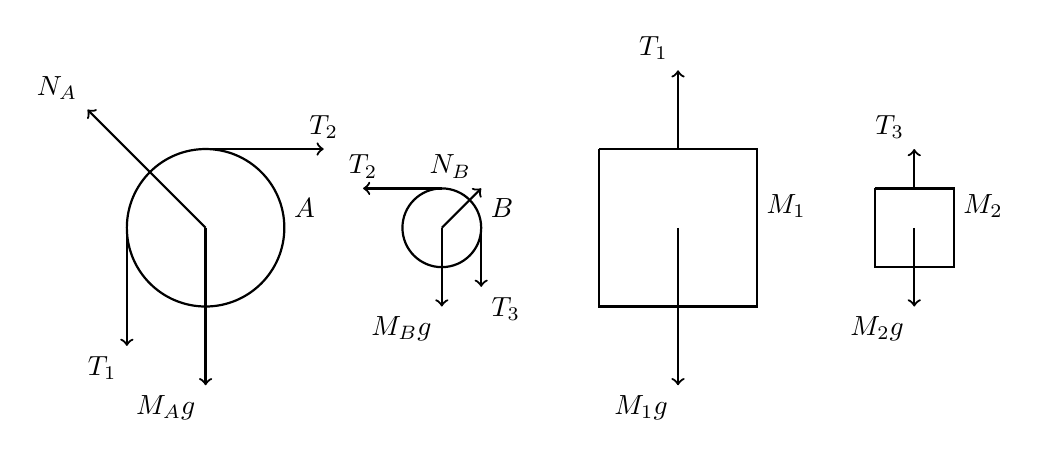
\begin{tikzpicture}
        \draw [thick] (-4.5,0) circle (1);
        \draw (-3.5,0) node[anchor=south west]{$A$};
        \draw [thick] (-1.5,0) circle (0.5);
        \draw (-1,0) node[anchor=south west]{$B$};
        \draw [thick] (0.5,1) -- (2.5,1) -- (2.5,-1) -- (0.5,-1) -- (0.5,1); 
        \draw (2.5,0) node[anchor=south west]{$M_1$};
        \draw [thick] (4,0.5) -- (5,0.5) -- (5,-0.5) -- (4,-0.5) -- (4,0.5);
        \draw (5,0) node[anchor=south west]{$M_2$};
        \draw [thick, ->] (-4.5,0) -- (-4.5,-2) node[pos=1,anchor=north
            east]{$M_Ag$};
        \draw [thick, ->] (-1.5,0) -- (-1.5,-1) node[pos=1,anchor=north
            east]{$M_Bg$};
        \draw [thick, ->] (1.5,0) -- (1.5,-2) node[pos=1,anchor=north
            east]{$M_1g$};
        \draw [thick, ->] (4.5,0) -- (4.5,-1) node[pos=1,anchor=north
            east]{$M_2g$};
        \draw [thick, ->] (1.5,1) -- (1.5,2) node[pos=1,anchor=south
            east]{$T_1$};
        \draw [thick, ->] (4.5,0.5) -- (4.5,1) node[pos=1,anchor=south
            east]{$T_3$};
        \draw [thick, ->] (-4.5,0) -- (-6,1.5) node[pos=1,anchor=south
            east]{$N_A$};
        \draw [thick, ->] (-1.5,0) -- (-1,0.5) node[pos=1,anchor=south
            east]{$N_B$};
        \draw [thick, ->] (-4.5,1) -- (-3,1) node[pos=1,anchor=south]{$T_2$};
        \draw [thick, ->] (-1.5,0.5) -- (-2.5,0.5)
            node[pos=1,anchor=south]{$T_2$};
        \draw [thick, ->] (-5.5,0) -- (-5.5,-1.5) node[pos=1,anchor=north
            east]{$T_1$};
        \draw [thick, ->] (-1,0) -- (-1,-0.75) node[pos=1,anchor=north
            west]{$T_3$};
        
    \end{tikzpicture}
\end{figure}

Write out Newton's 2nd Law for the pulleys and the blocks. Assuming the string
is non-extendable, the accelerations for all elements will be equal:
\begin{align*}
    I_{A}\frac{a}{R_{A}}&=T_{1}R_{A}-T_{2}R_{A}\\
    I_{B}\frac{a}{R_{B}}&=T_{2}R_{B}-T_{3}R_{B}\\
    M_{1}a&=M_{1}g-T_{1}\\
    M_{2}a&=T_{3}-M_{2}g
\end{align*}

Using row reduction, we can solve for $a$:
$$\left[
    \begin{array}{ccccc}
        R_{A} & -R_{A} & 0 & -\frac{1}{2}M_A R_A & 0\\
        0 & R_{B} & -R_{B} & -\frac{1}{2}M_B R_B & 0 \\
        -1 & 0 & 0 & -M_{1} & -M_{1}g\\
        0 & 0 & 1 & -M_{2} & M_{2}g
    \end{array}
\right]$$
$$\bm{a=\frac{2g(M_1+M_2)}{M_A+M_B+2M_1+2M_2}}$$

\section{Torque on a Triangle Frame}

\subsection*{Part A}

Draw the forces acting on the triangle:
\begin{figure}[H]
    \centering
    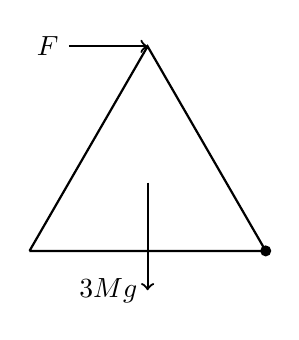
\begin{tikzpicture}
        \draw [thick] (0,0) -- (3,0) -- (1.5,2.598) -- (0,0);
        \draw [thick, ->] (0.5, 2.598) -- (1.5,2.598) node[pos=0,
            anchor=east]{$F$};
        \draw [thick, ->] (1.5, 0.866) -- (1.5, -0.5) node[pos=1,
            anchor=east]{$3Mg$};
        \fill (3,0) circle (2pt);
    \end{tikzpicture}
\end{figure}

Write Newton's 2nd Law for the triangle:
$$(3Mg)\left(\frac{L}{2}\right)-\left(F\frac{L\sqrt{3}}{2}\right)=I\alpha$$

Since we don't want the triangle to accelerate, $\alpha=0$:
\begin{align*}
    0&=(3Mg)\left(\frac{L}{2}\right)-\left(F\frac{L\sqrt{3}}{2}\right)\\
    \frac{FL\sqrt{3}}{2}&=\frac{3MgL}{2}\\
    F\sqrt{3}&=3Mg\\
    \bm{F}&\bm{=\frac{3Mg}{\sqrt{3}}}
\end{align*}

\subsection*{Part B}

We know that a parallel force supplied to a rotating object will cause zero
torque given from the definition of a cross product. As a result, the angle that
will cause the force to be parallel to the right leg will cause zero torque and
thus zero acceleration. 

$$\bm{\theta=60^{\circ}}$$

\section{Sore Back}

\subsection*{Part A}

\begin{figure}[H]
    \centering
    \includegraphics[scale=0.55]{"Figure 2"}
\end{figure}

Write out Newton's 2nd Law:
\begin{gather}
    \frac{2lF_{m}\sin(\alpha))}{3}-\frac{m_1gl\cos(\theta)}{2}-m_2gl\cos(\theta)-(F_{d}\sin(\beta))(0)=0\\
    -m_1g\cos(\theta)-m_2g\cos(\theta)+F_m\sin(\alpha)-F_d\sin(\beta)=0\\
    -m_1g\sin(\theta)-m_2g\sin(\theta)-F_m\cos(\alpha)+F_d\cos(\beta)=0
\end{gather}

Plugging in known values into equation 4:
\begin{align*}
    0&=\frac{2F_{m}\sin(\alpha))}{3}-\frac{m_1g\cos(\theta)}{2}-m_2g\cos(\theta)\\
    0&=\frac{2F_{m}\sin(12^{\circ}))}{3}-\frac{3(10\ \si{kg})(9.8\ \si{m\
    s^{-2}})\cos(30^{\circ})}{2}\\
    0&=0.138608F_{m}-127.306\ \si{kg\ m\ s^{-2}}\\
    \bm{F_{m}}&\bm{=918.46}\ \si{N}
\end{align*}

\subsection*{Part B}

Plugging in known values into equation 5:
\begin{align*}
    0&=-m_1g\cos(\theta)-m_2g\cos(\theta)+F_m\sin(\alpha)-F_d\sin(\beta)\\
    0&=-2(10\ \si{kg})(9.8\ \si{m\ s^{-2}})\cos(30^{\circ})+(918.46\
    \si{N})\sin(12^{\circ})-F_d\sin(\beta)\\
    0&=21.2176\ \si{N}-F_{d}\sin(\beta)\\
    F_{d}\sin(\beta)&=21.2176\ \si{N}
\end{align*}

Plugging in known values into equation 6:
\begin{align*}
    0&=-m_1g\sin(\theta)-m_2g\sin(\theta)-F_m\cos(\alpha)+F_d\cos(\beta)\\
    0&=-2(10\ \si{kg})(9.8\ \si{m\ s^{-2}})\sin(30^{\circ})-(918.46\
    \si{N})\cos(12^{\circ})+F_d\cos(\beta)\\
    0&=-996.389\ \si{N}+F_{d}\cos(\beta)\\
    F_{d}\cos(\beta)&=996.389\ \si{N}
\end{align*}

Dividing equation 5 by equation 6:
\begin{align*}
    \frac{F_{d}\sin(\beta)}{F_{d}\cos(\beta)}&=\frac{21.2176\ \si{N}}{996.389\ \si{N}}\\
    \tan(\beta)&=0.021294\\
    \bm{\beta}&\bm{=1.2199^{\circ}}
\end{align*}

Plugging $\beta$ into equation 5:
\begin{align*}
    F_{d}\sin(\beta)&=21.2176\ \si{N}\\
    F_{d}\sin(1.2199^{\circ})&=21.2176\ \si{N}\\
    F_{d}&=996.616\ \si{N}
\end{align*}

Divide by the weight of the person:
\begin{align*}
    \frac{F_{d}}{mg}&=\frac{996.616 \si{N}}{(50\ \si{kg})(9.8\ \si{m\ s^{-2}})}\\
    \bm{\frac{F_{d}}{mg}}&\bm{=2.0339}
\end{align*}

\subsection*{Part C}
Repeat steps in Parts A and B where $m_2=20\ \si{kg}$.
$$\bm{\frac{F_{d}}{mg}=3.3583}$$

\subsection*{Part D}
You should bend your knees rather than your back when you pick up a mass as this
will greatly lessen the torque on your back. Your weight of center of mass and
the mass you are picking up will be parallel to your back therefore producing no
torque. By bending your back, you are significantly increasing the forces on
your discs.

\section{Parson Standing on a Hill}

\subsection*{Part A}

Draw a free-body diagram for the hill:

\begin{figure}[H]
    \centering
    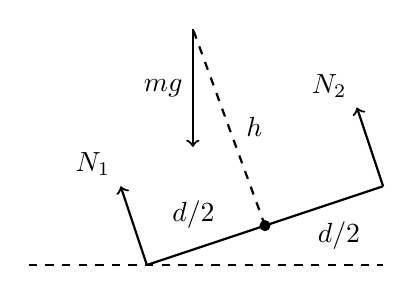
\begin{tikzpicture}
        \draw [thick] (0,0) -- (3,1) node[pos=0.68, anchor=north west]{$d/2$}
            node[pos=0.33, anchor=south east]{$d/2$};
        \draw [thick, dashed] (-1.5,0) -- (3,0);
        \draw [thick, ->] (0,0) -- (-0.333,1) node[anchor=south east]{$N_{1}$};
        \draw [thick, ->] (3,1) -- (2.667,2) node[anchor=south east]{$N_{2}$};
        \draw [thick, dashed] (1.5,0.5) -- (0.5833,3) node[pos=0.4, anchor=south
            west]{$h$};
        \fill (1.5,0.5) circle (2pt);
        \draw [thick, ->] (0.5833,3) -- (0.5833, 1.5) node[pos=0.5,
            anchor=east]{$mg$};
    \end{tikzpicture}
\end{figure}

Halfway reduced:

\begin{figure}[H]
    \centering
    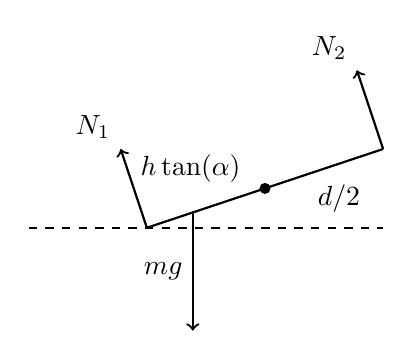
\begin{tikzpicture}
        \draw [thick] (0,0) -- (3,1) node[pos=0.68, anchor=north west]{$d/2$}
            node[pos=0.44, anchor=south east]{$h\tan(\alpha)$};
        \draw [thick, dashed] (-1.5,0) -- (3,0);
        \draw [thick, ->] (0,0) -- (-0.333,1) node[anchor=south east]{$N_{1}$};
        \draw [thick, ->] (3,1) -- (2.667,2) node[anchor=south east]{$N_{2}$};
        \draw [thick, ->] (0.5833,0.1944) -- (0.5833, -1.3056) node[pos=0.5,
            anchor=east]{$mg$};
        \fill (1.5,0.5) circle (2pt);
    \end{tikzpicture}
\end{figure}

Fully reduced (ignoring the horizontal component of $mg$ because it is cancelled
by friction):

\begin{figure}[H]
    \centering
    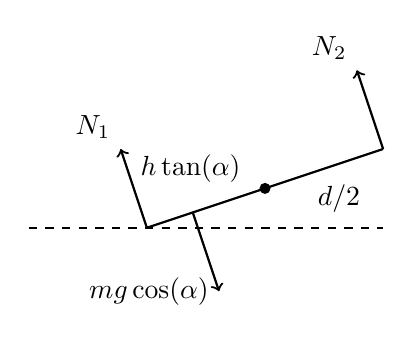
\begin{tikzpicture}
        \draw [thick] (0,0) -- (3,1) node[pos=0.68, anchor=north west]{$d/2$}
            node[pos=0.44, anchor=south east]{$h\tan(\alpha)$};
        \draw [thick, dashed] (-1.5,0) -- (3,0);
        \draw [thick, ->] (0,0) -- (-0.333,1) node[anchor=south east]{$N_{1}$};
        \draw [thick, ->] (3,1) -- (2.667,2) node[anchor=south east]{$N_{2}$};
        \draw [thick, ->] (0.5833,0.1944) -- (0.9166, -0.8056) node[pos=1,
            anchor=east]{$mg\cos(\alpha)$};
        \fill (1.5,0.5) circle (2pt);
    \end{tikzpicture}
\end{figure}

Write out Newton's 2nd Law:
\begin{gather}
    N_{1}+N_{2}-mg\cos(\alpha)=0\\
    -\frac{N_{1}d}{2}+\frac{N_{2}d}{2}+(mg\cos(\alpha))(h\tan(\alpha))=0
\end{gather}

Multiply equation 8 by $-2/d$ and solve for $N_{1}$ via elimination:
\begin{align*}
    0&=N_{1}-N_{2}-\frac{2mgh\sin(\alpha)}{d}\\
    0&=2N_{1}-\frac{2mgh\sin(\alpha)}{d}-mg\cos(\alpha)\\
    N_{1}&=\frac{mg\cos(\alpha)}{2}+\frac{mgh\sin(\alpha)}{d}\\
    \bm{N_{1}}&\bm{=\frac{mg(d\cos(\alpha)+2h\sin(\alpha))}{2d}}
\end{align*}


Multiply equation 8 by $2/d$ and solve for $N_{2}$ via elimination:
\begin{align*}
    0&=-N_{1}+N_{2}+\frac{2mgh\sin(\alpha)}{d}\\
    0&=2N_{2}+\frac{2mgh\sin(\alpha)}{d}-mg\cos(\alpha)\\
    N_{2}&=\frac{mg\cos(\alpha)}{2}-\frac{mgh\sin(\alpha)}{d}\\
    \bm{N_{2}}&\bm{=\frac{mg(d\cos(\alpha)-2h\sin(\alpha))}{2d}}
\end{align*}

\subsection*{Part B}

Solve $N_{2}=0$ for $d$:
\begin{align*}
    0&=\frac{mg\cos(\alpha)}{2}-\frac{mgh\sin(\alpha)}{d}\\
    \frac{mgh\sin(\alpha)}{d}&=\frac{mg\cos(\alpha)}{2}\\
    d&=\frac{2mgh\sin(\alpha)}{mg\cos(\alpha)}\\
    \bm{d}&\bm{=2h\tan(\alpha)}
\end{align*}

\end{document}
